\documentclass[tikz,border=10pt]{standalone}
\usepackage{tikz}
\usetikzlibrary{positioning, shadows, calc}

\begin{document}
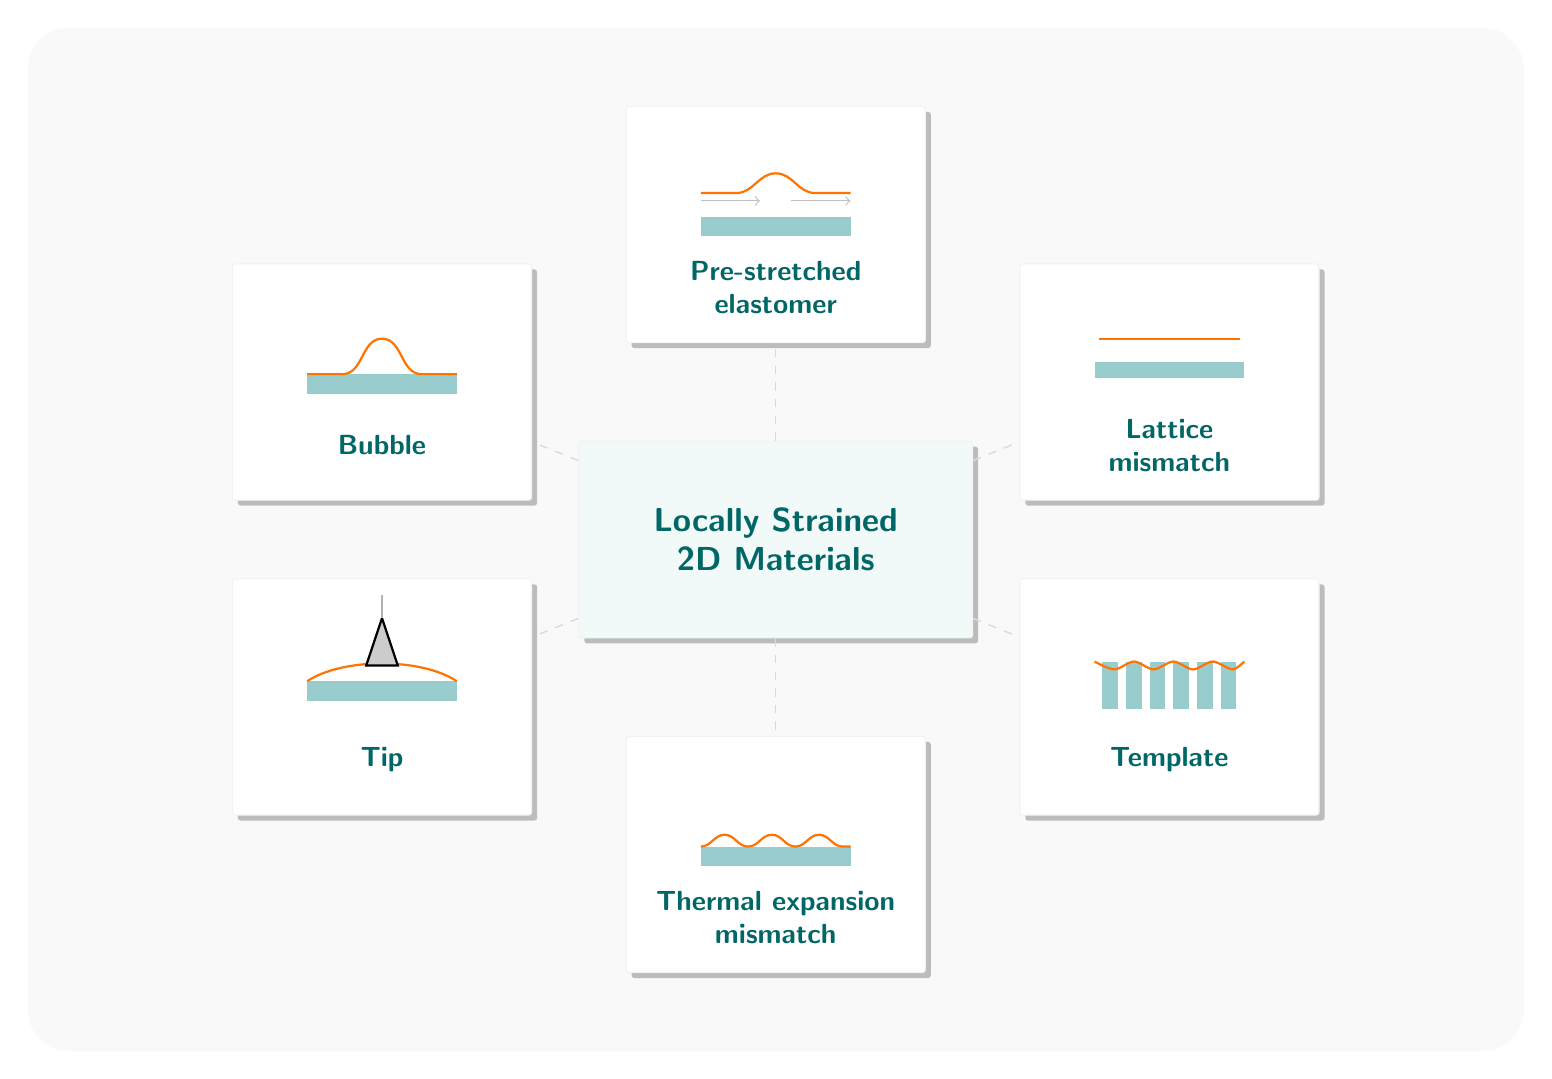
\begin{tikzpicture}[
    font=\sffamily\bfseries,
    method/.style={text=teal!80!black, align=center},
    panel/.style={draw=gray!10, fill=white, drop shadow={shadow xshift=0.7mm, shadow yshift=-0.7mm}, 
                  rounded corners=1pt, minimum width=3.8cm, minimum height=3cm},
    connection/.style={draw=gray!30, line width=0.5pt, dashed}
]

% Light background
\fill[gray!5, rounded corners=15pt] (-9.5,-6.5) rectangle (9.5,6.5);

% Central node
\node[panel, fill=teal!5, minimum width=5cm, minimum height=2.5cm] (center) at (0,0) {};
\node[align=center, font=\sffamily\bfseries\large, text=teal!80!black] at (0,0) {Locally Strained\\2D Materials};

% Panels layout
\node[panel] (p1) at (0,4) {};
\node[panel] (p2) at (-5,2) {};
\node[panel] (p3) at (-5,-2) {};
\node[panel] (p4) at (0,-4) {};
\node[panel] (p5) at (5,-2) {};
\node[panel] (p6) at (5,2) {};

% Dotted connections
\foreach \i in {1,...,6} {
    \draw[connection] (center) -- (p\i);
}

% Pre-stretched elastomer
\begin{scope}[shift={(0,4.3)}]
    \draw[gray!50,->] (-0.95,0) -- (-0.2,0);
    \draw[gray!50,<-] (0.95,0) -- (0.2,0);
    \fill[teal!40] (-0.95,-0.2) rectangle (0.95,-0.45);
    \draw[orange!90!red, thick] (-0.95,0.1) -- (-0.5,0.1) to[out=0,in=180] (0,0.35)
                               to[out=0,in=180] (0.5,0.1) -- (0.95,0.1);
\end{scope}
\node[method] at (0,3.2) {Pre-stretched\\elastomer};

% Bubble
\begin{scope}[shift={(-5,2.3)}]
    \fill[teal!40] (-0.95,-0.45) rectangle (0.95,-0.2);
    \draw[orange!90!red, thick] (-0.95,-0.2) -- (-0.5,-0.2) to[out=0,in=180] (0,0.25)
                               to[out=0,in=180] (0.5,-0.2) -- (0.95,-0.2);
\end{scope}
\node[method] at (-5,1.2) {Bubble};

% Tip (corrected to indentation)
\begin{scope}[shift={(-5,-1.6)}]
    \fill[teal!40] (-0.95,-0.45) rectangle (0.95,-0.2);
    \draw[orange!90!red, thick] (-0.95,-0.2) .. controls (-0.5,0.1) and (0.5,0.1) .. (0.95,-0.2);
    \draw[black, thick, fill=gray!40] (0,0.6) -- (-0.2,0) -- (0.2,0) -- cycle;
    \draw[gray!60, thick] (0,0.6) -- (0,0.9);
\end{scope}
\node[method] at (-5,-2.8) {Tip};

% Thermal expansion mismatch
\begin{scope}[shift={(0,-3.7)}]
    \fill[teal!40] (-0.95,-0.45) rectangle (0.95,-0.2);
    \draw[orange!90!red, thick] (-0.95,-0.2) 
        to[out=0,in=180] (-0.65,-0.05) 
        to[out=0,in=180] (-0.35,-0.2) 
        to[out=0,in=180] (-0.05,-0.05) 
        to[out=0,in=180] (0.25,-0.2) 
        to[out=0,in=180] (0.55,-0.05) 
        to[out=0,in=180] (0.85,-0.2) 
        to[out=0,in=180] (0.95,-0.2);
\end{scope}
\node[method] at (0,-4.8) {Thermal expansion\\mismatch};

% Template (corrected to conformal grating)
\begin{scope}[shift={(5,-1.7)}]
    \foreach \x in {-0.75,-0.45,-0.15,0.15,0.45,0.75} {
        \fill[teal!40] (\x-0.1,-0.45) rectangle (\x+0.1,0.15);
    }
    \draw[orange!90!red, thick, smooth] plot coordinates {
        (-0.95,0.15) (-0.7,0.05) (-0.45,0.15) (-0.2,0.05)
        (0.05,0.15) (0.3,0.05) (0.55,0.15) (0.8,0.05) (0.95,0.15)
    };
\end{scope}
\node[method] at (5,-2.8) {Template};

% Lattice mismatch (corrected as stacked lattices)
\begin{scope}[shift={(5,2.3)}]
    \fill[teal!40] (-0.95,-0.25) rectangle (0.95,-0.05);
    \draw[orange!90!red, thick] (-0.9,0.25) -- (-0.6,0.25) -- (-0.3,0.25) -- (0,0.25)
                                -- (0.3,0.25) -- (0.6,0.25) -- (0.9,0.25);
\end{scope}
\node[method] at (5,1.2) {Lattice\\mismatch};

\end{tikzpicture}
\end{document}
